\documentclass[main.tex]{subfiles}
\newcommand\chapterlabel{Ch-equilibrium}\setcounter{figurenewcounter}{0}\setcounter{tablenewcounter}{0}\setcounter{formulanewcounter}{0}


\begin{document}
%\linenumbers
%\setcounter{chapter}{5}
  
   \import{../\chapterlabel/files/}{ChapterName}
%\label{ch:atoms}


      \begin{marginfigure}
      \begin{tikzpicture} \node (a) at (0,0) {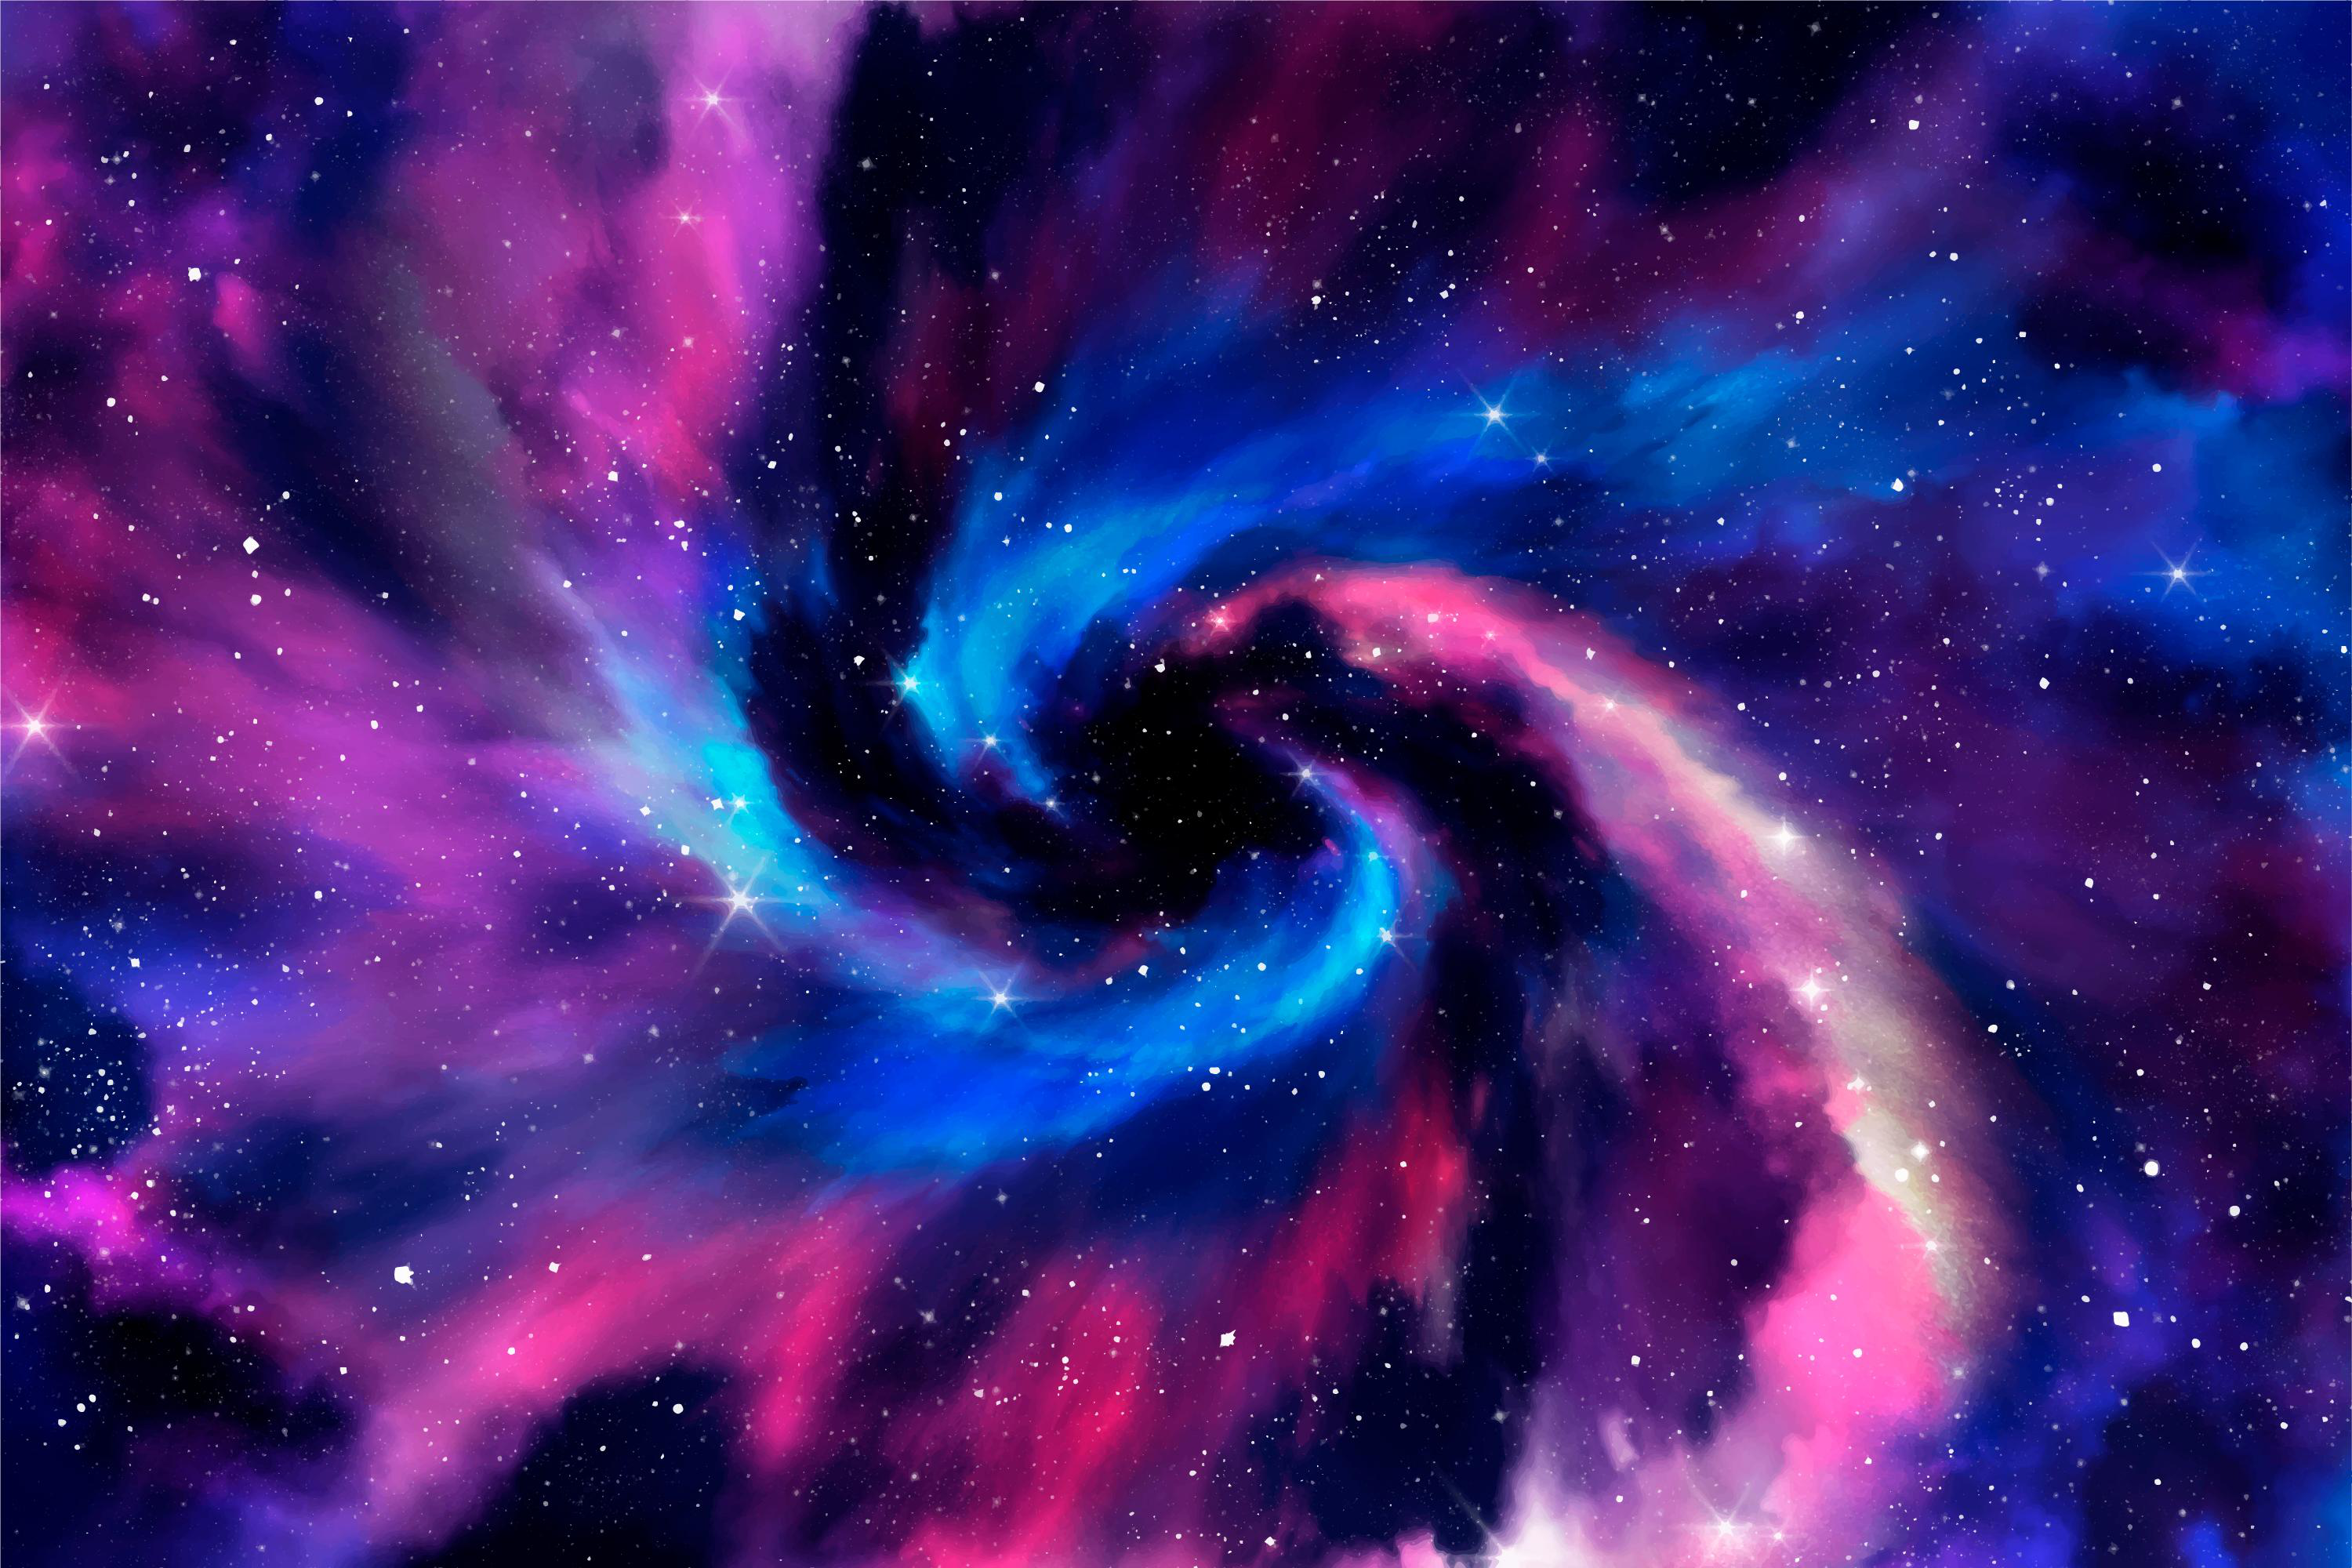
\includegraphics[width=4cm]{../Ch-equilibrium/figure1}} node[rotate=90, font=\tiny] at ([yshift=.5cm,xshift=.1cm]a.south east) {\textsuperscript{\textcopyright} PxFuel} ;
\end{tikzpicture}
\end{marginfigure}
   \import{../\chapterlabel/files/}{ChapterIntro}




\begin{marginfigure}%LEARNING GOALS BOX
\begin{mytcbox}{GOALS}
\begin{enumerate}[label=\protect\circled{\color{white}\arabic*}]
\item Formulate equilibrium constants
\item Interconvert $K_c$ and $K_p$
\item Apply Le Ch\^{a}telier
\item Interpret the magnitude of $K_c$
\item Carry simple equilibrium calculations
\end{enumerate}
\end{mytcbox}
\vspace{1cm}
\begin{tcolorbox}[enhanced,colback=red!5!white,colframe=black!50!red,boxrule=1pt,
  arc=0pt,outer arc=0pt,drop heavy lifted shadow]
\faGears\ 
\docenvdef{Discussion:}  \import{../\chapterlabel/files/}{ChapterDiscussion}


\end{tcolorbox}
\end{marginfigure}%LEARNING GOALS BOX

\section{Chemical Equilibrium} \import{../\chapterlabel/files/}{SectionIntro-Chemical-Equilibrium}

\sloppy\begin{description}

\item[\docfilehook{Forward and reverse reactions}{}] \import{../\chapterlabel/files/}{SubSection-Chemical-Equilibrium-Forward-and-reverse-reactions}




\item[\docfilehook{Equilibrium}{}] \import{../\chapterlabel/files/}{SubSection-Chemical-Equilibrium-Equilibrium}




\import{../\chapterlabel/files/}{SideFigure-Forward-and-reverse-reactions}




\item[\docfilehook{Equilibrium and concentration}{}] \import{../\chapterlabel/files/}{SubSection-Chemical-Equilibrium-Equilibrium-and-concentration}



  \import{../\chapterlabel/problems/}{SampleProblem1}






\end{description}

 
\section{{The equilibrium constant}}   \import{../\chapterlabel/files/}{SectionIntro-The-equilibrium-constant}

\sloppy\begin{description}



\item[\docfilehook{Equilibrium mixtures}{}] \import{../\chapterlabel/files/}{SubSection-The-equilibrium-constant-Equilibrium-mixtures}



 \import{../\chapterlabel/files/}{Table-Kc-and-reactions}\newpage
\import{../\chapterlabel/files/}{Figure-Equilibrium}

\item[\docfilehook{The equilibrium constant of a reaction}{}] \import{../\chapterlabel/files/}{SubSection-The-equilibrium-constant-The-equilibrium-constant-of-a-reaction}



  \import{../\chapterlabel/problems/}{SampleProblem2}

\import{../\chapterlabel/files/}{SideFigure-Meaning-of-Kc}






\item[\docfilehook{Equilibrium constant expression}{}] \import{../\chapterlabel/files/}{SubSection-The-equilibrium-constant-Equilibrium-constant-expression}

 
\item[\docfilehook{Equilibrium involving solids, liquids and solutions}{}] \import{../\chapterlabel/files/}{SubSection-The-equilibrium-constant-Equilibrium-involving-solids-liquids-and-solutions}


  \import{../\chapterlabel/problems/}{SampleProblem3}


\item[\docfilehook{Equilibrium constant in terms of pressures}{}] \import{../\chapterlabel/files/}{SubSection-The-equilibrium-constant-Equilibrium-constant-in-terms-of-pressures}



\item[\docfilehook{Relating $K_{c}$ and $K_{p}$}{ }] \import{../\chapterlabel/files/}{SubSection-The-equilibrium-constant-Relating-Kc-and-Kp}



\end{description}
  \import{../\chapterlabel/problems/}{SampleProblem4}











\section{ {Using equilibrium constants}}   \import{../\chapterlabel/files/}{SectionIntro-Using-equilibrium-constants}



   
   \sloppy
\begin{description}
\item[\docfilehook{Solving from $K_c$}{}]\import{../\chapterlabel/files/}{SubSection-Using-equilibrium-constants-Solving-from-Kc}



  \import{../\chapterlabel/problems/}{SampleProblem5}
\end{description}
 



\section{ Concentration or pressure ratio}
   \import{../\chapterlabel/files/}{SectionIntro-Concentration-or-pressure-ratio}
\sloppy\begin{description}

\item[\docfilehook{Definition of concentration ratio	}{}] \import{../\chapterlabel/files/}{SubSection-Concentration-or-pressure-ratio-Definition-of-concentration-ratio}



\item[\docfilehook{Use of concentration ratios	}{}] \import{../\chapterlabel/files/}{SubSection-Concentration-or-pressure-ratio-Use-of-concentration-ratios}


\end{description}
  \import{../\chapterlabel/problems/}{SampleProblem6}










\import{../\chapterlabel/files/}{SideFigure-Image-of-le-chatelier}

\section{ {Le Ch\^{a}telier principle}}
   \import{../\chapterlabel/files/}{SectionIntro-Le-Chatelier-principle}

\sloppy\begin{description}
\item[\docfilehook{Le Ch\^{a}telier principle}{}] \import{../\chapterlabel/files/}{SubSection-Le-Chatelier-principle-Le-Chatelier-principle}


 \item[\docfilehook{Change in concentration}{}] \import{../\chapterlabel/files/}{SubSection-Le-Chatelier-principle-Change-in-concentration}


 


\import{../\chapterlabel/files/}{SideFigure-Le-chatelier}



 \item[\docfilehook{Temperature change}{}] \import{../\chapterlabel/files/}{SubSection-Le-Chatelier-principle-Temperature-change}



 


\newpage
  \item[\docfilehook{Volume change}{}] 
\import{../\chapterlabel/files/}{SubSection-Le-Chatelier-principle-Volume-change}

   \import{../\chapterlabel/files/}{Table-Le-chatelier}
 
\end{description}





  \import{../\chapterlabel/problems/}{SampleProblem7}





\end{document}
